\documentclass{article}
\usepackage[utf8]{inputenc}
\usepackage{graphicx}

\newcommand{\TODO}[1]{\textcolor{red}{\textbf{[TODO:#1]}}}
\newcommand{\symb}[1]{\textit{#1}} 

\title{Static optimization of memory consistency checks in heterogeneous computations by performance model propagation}

\author{Christoph Kessler, Ludovic Henrio and ... }

\date{November 2019}

\begin{document}

\maketitle

\begin{abstract}
    We propose a static analysis of multi-variant kernel programs for
    heterogeneous systems with distributed memory
    and a coherent software caching of accessed
    data elements in device memory.
    In such systems, the kernels can execute either
    on the host (e.g., a CPU) or on the device
    (e.g., a GPU), depending on a performance
    model that predicts the fastest unit based
    on data size and location.
    Our analysis works by an abstract interpretation
    of the program's flow graph, propagating 
    kernel and data transfer performance models 
    along the graph in order to approximate the
    dynamic data locations at any static program point.
    We show how this information
    allows to identify and 
    eliminate a safe subset of redundant
    checks for element accesses in the software
    cache coherence protocol.
    
\end{abstract}
\section{Introduction}

Idea: abstract interpretation with an adequate abstract domain.
Adequate for anticipating where data is located and where computation will occur.
THEN must be compliant with the cost model / the way we can compute/predict where computation will occur.

Somehow we will need an abstraction of the function that computes where computation occurs, i.e. of the function that computes which variant of the function should be called for the considered parameters of the call.

TODO:

- motivating example or scenario. 
Maybe along the lines of Figure~\ref{fig:DAG}?

- investigate possible representation of abstract representation of data. see if this is good enough to have an approximation of the function that computes where computation occurs, then investigate relational abstract domain, at least based on the size (intervals) of the original data-set.
- see how to compute an abstraction of the performance model.


- see how to compute an abstraction of the performance model.

\begin{figure}
    \centering
    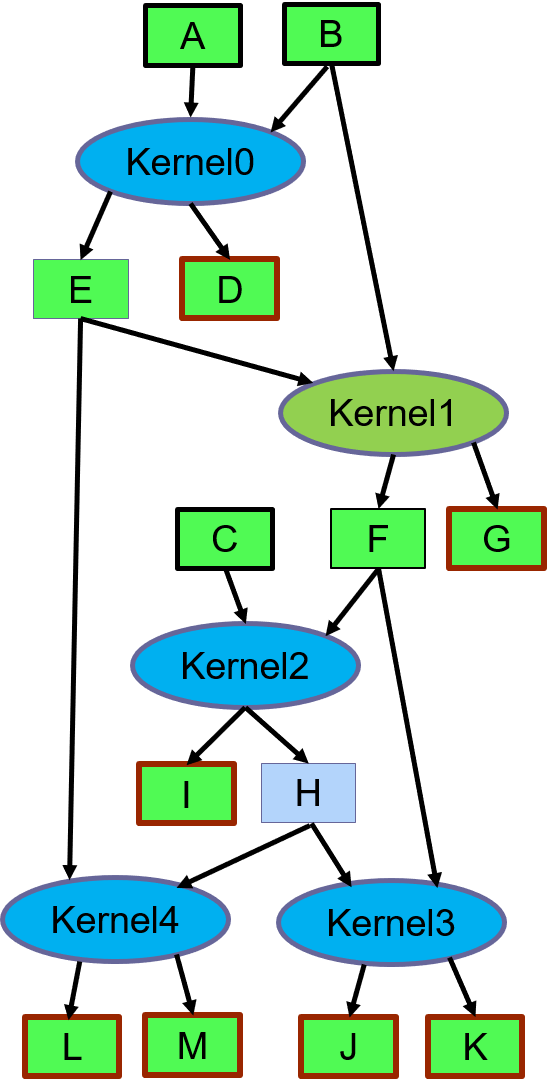
\includegraphics[width=0.3\textwidth]{DAG2.png}\hfill
    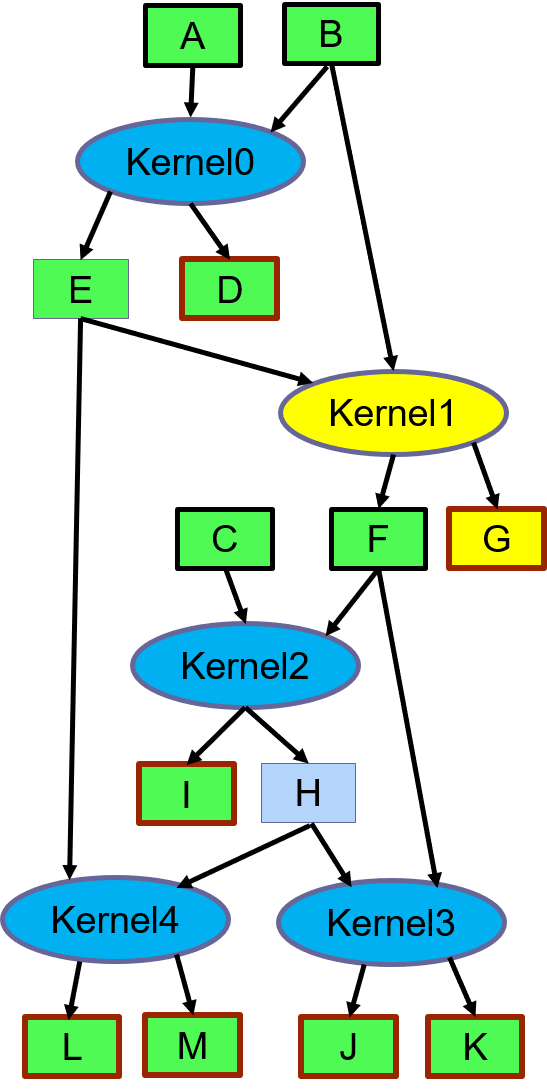
\includegraphics[width=0.3\textwidth]{DAG1.png}\hfill
    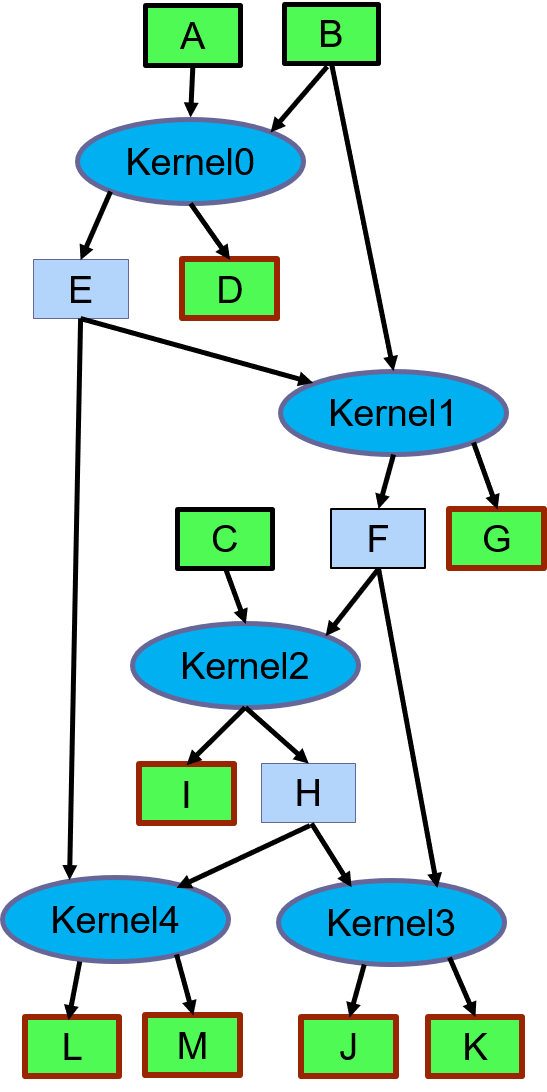
\includegraphics[width=0.3\textwidth]{DAG0.png}
    
    \caption{Example data flow graph with multi-variant kernel calls (ovals) and operand containers (rectangles). Operands live on entry (exit) are indicated by a blue (brown) frame. The fill colors for kernel calls indicate the executing unit (yellow: CPU, blue: GPU, green: statically unknown). For operand containers, yellow (blue) containers need only be allocated in main memory (device memory), while green containers may need both. --- Left: For Kernel 1 it is not statically known whether it will be executed on CPU or GPU. Middle: We know by refined static analysis that Kernel 1 will execute on CPU and, hence, that output operand $G$ needs not be downloaded. Right: We know statically that Kernel 2
    will execute on GPU, hence output operand $F$ can reside in device memory only. Given a mapping of the kernel calls to execution units, operand storage and requirements for data transfer can then be inferred statically \cite{Kessler:SCOPES19}.}
    \label{fig:DAG}
\end{figure}


\section{Problem formalization}

\subsection{Architecture model}

We consider a heterogeneous system consisting of
a host processing unit (usually, a CPU) and 
a programmable accelerator (e.g., a GPU) with separate device memory,
attached via PCIe bus or similar network.
A generalization to more than two execution
units can be done later.

\subsection{Program model}

For the program representation 
we use a bipartite DAG model \cite{Kessler:SCOPES19}.
% from the SCOPES'19 paper.

We model a program as a bipartite
graph consisting of $N$ calls to multi-variant 
kernels and $m$ operand data containers as nodes.
The kernel calls, 
numbered $i=1,...N$ in execution order,
are pre-mapped to CPU ($d_i=0$) or GPU ($d_i=1$).
Each kernel call takes a small constant number
$I_i$ of input operand containers and produces
$O_j$ output containers. Edges link input operand
containers to the kernel calls using them, 
as well as kernel calls to the output operand
containers they produce. The data flow via
containers is acyclic, which implies that each
container is written exactly once 
(static single-assignment property). 

...

Start from a DAG with green kernels (unknown where
executed) and try to infer the color (blue or yellow)
from static analysis if the range of input sizes
is narrowed.


Do it for now for a
sequence (for now) of calls to multi-variant
functions operating on data containers (vectors, matrices etc.). Each multi-variant function has
different implementations for the different
units in the heterogeneous system.
Execution time behavior for each variant is
assumed to be known as a function in the
data size and location. There will be an
intersection point below which CPU implementations
dominate GPU implementations and above which it is
vice versa.


No loops, no conditions, just sequences.

\subsection{Performance model}

For each kernel $i$ executing on device $d_i$,
a function $t_{i,d_i}(N_1,...,N_{I_i})$
indicates the kernel execution time
(excluding data transfers). 

Let $t_{comm}(N)$ denote the cost to communicate
a block of $N$ elements. We can expect that,
at least in theory, $t_{comm}(N)$ is linear in $N$.
\footnote{This is the expected overall trend. In practice, anomalies can occur for certain data sizes
\cite{Kessler:SCOPES19}, for
example because data transfer functions e.g.\ in 
CUDA can internally use different data transfer protocols for different data sizes. Likewise,
the communication cost might be asymmetric,
i.e., the time per KB might differ for uploads and downloads; however, the generalization of our
approach to such elaboration of the
performance model is straightforward.}



\subsection{Execution model}

The execution model determines when and how
the variant to be executed will be decided.

(a) \emph{Greedy selection}, considering one call at a time (in program order) and deciding what is locally best considering the input size and locations that are a consequence of the preceding decisions. In other words, we apply the HEFT heuristic \cite{HEFT}. This is what we will consider for now in this paper, for simplicity.
Can lead to a globally suboptimal solution.

(b) \emph{Optimal (global) selection}, cf.\ Hansson and Kessler \cite{Hansson2015}.
This decides the selection for all calls 
together, thus taking all effects of these
decisions on state
(data locations) into account.

\subsection{Data and memory model}

For the operand arrays, 
we use \emph{smart data-containers} 
\cite{Dastgeer2016}
for array-based generic data types 
with a STL-compliant interface such as \verb+Vector<...>+ that wrap
the elements array and metadata, and internally
perform optimizations such as software caching
of container elements with (where desired)
sequentially consistent memory access.


\section{Abstract Interpretation}

\bibliographystyle{IEEEtran}
\bibliography{references}

\end{document}
